\chapter{数値解析例}
本研究では,全ての解析問題を線形弾性問題として解析を行った.連立一次方程式の求解には
共役勾配法(Conjurate Gradient Method, CG法)を用いており,
収束判定のしきい値を相対残差で$10^{-13}$とした.

\section{3次の基底関数を用いたIGA解析}
通常のIGA解析を行い,2次と
3次の基底関数を用いた解析の誤差精度の検証を行った.

\subsection{内圧を受ける厚肉円筒の解析}
解析対象は,外径$4\ $mm,内径$2\ $mmの厚肉円筒であり,解析には二次元の$1/4$モデルを使用した.
解析問題を図~\ref{fig:internal pressure}に示す.
平面ひずみ状態を仮定し,ヤング率は$206\ $GPa,ポアソン比は$0.3$とし,
数値積分には各方向の積分点数が$4\times 4$のガウス・ルジャンドル積分法を用いた.

\begin{figure}[htbp]
  \centering
  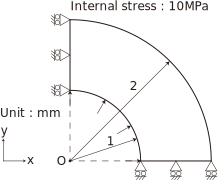
\includegraphics[keepaspectratio, scale = 0.85]
  {fig/内圧を受ける厚肉円筒モデル.ai}
  \caption{Analytical model of thick cylinder subjected to internal pressure}
  \label{fig:internal pressure}
\end{figure}

図~\ref{fig:internal pressure}に示すようにパラメータ空間を設定した.
2次の基底関数を用いた場合と3次の基底関数を用いた場合で,
パラメータ空間の各方向に対してコントロールポイント数が等しく,
一様オープンノットベクトルのIGA解析モデルをそれぞれ作成し,
各方向のコントロールポイントの分割数を変更したIGA解析モデルを作成した.
各方向のコントロールポイント数,自由度数,総要素数を表~\ref{table:ip}に示す.

\begin{table}[hbtp]
  \caption{Details of IGA analytical model}
  \label{table:ip}
  \centering
  \scalebox{0.95}{
    \begin{tabular}{|c|c|c|c|c|c|c|c|c|}
      \hline
      Order of basis function & \multicolumn{4}{c|}{2} & \multicolumn{4}{c|}{3} \\
      \hline
      Control points ($\xi \times \eta$) & $5\times 5$ & $10\times 10$ & $20\times 20$ & $40\times 40$ & $5\times 5$ & $10\times 10$ & $20\times 20$ & $40\times 40$ \\
      \hline
      Degrees of freedom & 40 & 180 & 760 & 3120 & 40 & 180 & 760 & 3120 \\
      \hline
      Total elements & 9 & 64 & 324 & 1444 & 4 & 49 & 289 & 1369 \\
      \hline
    \end{tabular}
  }
\end{table}

\newpage

例として,2次の基底関数と3次の基底関数で,各方向のコントロールポイント数が$5\times 5$のIGA解析モデルを
図~\ref{fig:iga order 2}及び図~\ref{fig:iga order 3}に示す.
点がコントロールポイント,実線が要素境界を表しており,
一様オープンノットベクトルを用いているため,各方向に等間隔の要素分割となっている.

\begin{figure}[htbp]
  \begin{tabular}{cc}
    \begin{minipage}[t]{0.45\hsize}
      \centering
      \includegraphics[keepaspectratio, scale=0.3]
      {fig/result_data_etc/iga/order2/model.png}
      \caption{An example of second-order analytical model (Control points $5\times 5$)}
      \label{fig:iga order 2}
    \end{minipage} &
    \begin{minipage}[t]{0.45\hsize}
      \centering
      \includegraphics[keepaspectratio, scale=0.3]
      {fig/result_data_etc/iga/order3/model.png}
      \caption{An example of third-order analytical model (Control points $5\times 5$)}
      \label{fig:iga order 3}
    \end{minipage}
  \end{tabular}
\end{figure}

\noindent
以上の解析モデルについて解析を行い,精度検証を行った.

内圧$P\ $MPaを受ける内径$2r_1\ $mm,外径$2r_2\ $mmの厚肉円筒の
応力の理論解は,円筒の中心を原点とした極座標表記で以下のように表される.

\begin{align}
  \sigma_{rr} &= -\frac{{r_1}^2{r_2}^2P}{{r_2}^2-{r_1}^2}\frac{1}{r^2}
              +\frac{{r_1}^2P}{{r_2}^2-{r_1}^2}\\
  \sigma_{\theta\theta} &= \frac{{r_1}^2{r_2}^2P}{{r_2}^2-{r_1}^2}\frac{1}{r^2}
                   +\frac{{r_1}^2P}{{r_2}^2-{r_1}^2}
\end{align}

\noindent
この理論解を用いて解析結果の誤差ノルムを算出し,
誤差精度の比較を行った.
誤差ノルムは以下のように定義した.

\begin{equation}
  {\rm{Error\ norm}} = \frac{\sqrt{\int_{\Omega}(\alpha_{\rm{analysis}}-\alpha_{\rm{theory}})^2 d\Omega}}{\sqrt{\int_{\Omega}{\alpha_{\rm{theory}}}^2 d\Omega}}
\end{equation}

\noindent
ここで,$\Omega$はIGA解析モデル全体の領域,
$\alpha$は比較パラメータである半径方向応力$\sigma_{rr}$,周方向応力$\sigma_{\theta\theta}$であり,
$\alpha_{\rm{theory}}$は比較パラメータの理論解,$\alpha_{\rm{analysis}}$は比較パラメータの解析結果の数値を表している.

\newpage

IGA解析結果の変位分布図を示す.
図~\ref{fig:iga 01}~図~\ref{fig:iga 04}は2次の基底関数と3次の基底関数の半径方向変位$u_{r}$である.

\begin{figure}[htbp]
  \begin{tabular}{cc}
    \begin{minipage}[t]{0.45\hsize}
      \centering
      \includegraphics[keepaspectratio, scale=0.3]
      {fig/result_data_etc/iga/order2/2_5x5.png}
      \caption{Displacement in r direction of second-order analytical model (Control points $5\times 5$)}
      \label{fig:iga 01}
    \end{minipage} &
    \begin{minipage}[t]{0.45\hsize}
      \centering
      \includegraphics[keepaspectratio, scale=0.3]
      {fig/result_data_etc/iga/order3/3_5x5.png}
      \caption{Displacement in r direction of third-order analytical model (Control points $5\times 5$)}
      \label{fig:iga 02}
    \end{minipage}
  \end{tabular}
\end{figure}

\begin{figure}[htbp]
  \begin{tabular}{cc}
    \begin{minipage}[t]{0.45\hsize}
      \centering
      \includegraphics[keepaspectratio, scale=0.3]
      {fig/result_data_etc/iga/order2/2_40x40.png}
      \caption{Displacement in r direction of second-order analytical model (Control points $40\times 40$)}
      \label{fig:iga 03}
    \end{minipage} &
    \begin{minipage}[t]{0.45\hsize}
      \centering
      \includegraphics[keepaspectratio, scale=0.3]
      {fig/result_data_etc/iga/order3/3_40x40.png}
      \caption{Displacement in r direction of third-order analytical model (Control points $40\times 40$)}
      \label{fig:iga 04}
    \end{minipage}
  \end{tabular}
\end{figure}

半径方向応力$\sigma_{rr}$と周方向応力$\sigma_{\theta\theta}$の誤差ノルムを算出し,
2次の基底関数を用いた場合と3次の基底関数を用いた場合の
自由度数と誤差ノルムの関係を両対数グラフで図~\ref{fig:iga ER 01},図~\ref{fig:iga ER 02}に示す.

\begin{figure}[htbp]
  \centering
  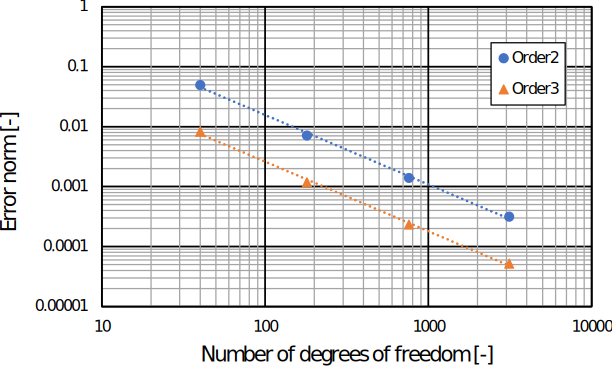
\includegraphics[keepaspectratio, scale = 0.8]
  {fig/result_data_etc/iga/ER01-crop.pdf}
  \caption{Error norm of $\sigma_{rr}$}
  \label{fig:iga ER 01}
\end{figure}

\begin{figure}[htbp]
  \centering
  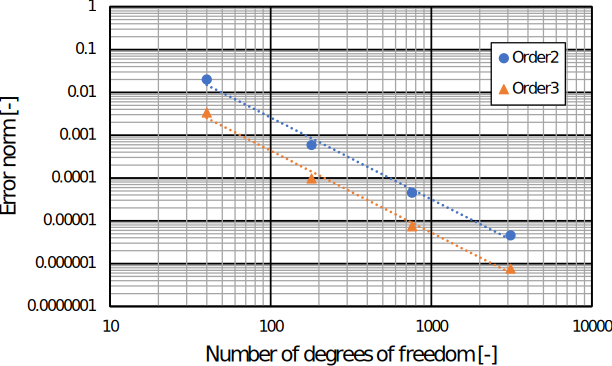
\includegraphics[keepaspectratio, scale = 0.8]
  {fig/result_data_etc/iga/ER02-crop.pdf}
  \caption{Error norm of $\sigma_{\theta\theta}$}
  \label{fig:iga ER 02}
\end{figure}

\newpage

\section{3次の基底関数を用いた重合パッチ法解析}
重合パッチ法解析を行い,2次と
3次の基底関数を用いた解析の誤差精度の検証を行った.

\subsection{遠方で一様引張を受ける円孔を有する平板の解析}

解析対象は,中央に半径$1\ $mmの円孔を有する遠方で一様引張を受ける平板であり,解析には二次元の$1/4$モデルを使用した.
解析問題を図~\ref{fig:GL}に示す.
平面ひずみ状態を仮定し,ヤング率は$206\ $GPa,ポアソン比は$0.3$とした.

\begin{figure}[htbp]
  \centering
  \includegraphics[keepaspectratio, scale = 0.85]
  {fig/GL.ai}
  \caption{Analytical model of plate with a circular hole}
  \label{fig:GL}
\end{figure}

\noindent
図~\ref{fig:GL}の問題は重合パッチ法では図~\ref{fig:G_and_L}に示す解析モデルと等価である.

\begin{figure}[htbp]
  \centering
  \includegraphics[keepaspectratio, scale = 0.85]
  {fig/G_and_L.ai}
  \caption{Analytical model of Global patch and Local patch}
  \label{fig:G_and_L}
\end{figure}

\newpage

\noindent
グローバルパッチはシンプルな形状を作成し,一様引張と対称性を表すための変位固定の境界条件を設定した.
ローカルパッチは円孔を表現する詳細形状を作成し,グローバルパッチ上のローカルパッチの境界$\Gamma^{GL}$で変位固定を行った.

数値積分には各方向の積分点数が$4\times 4$のガウス・ルジャンドル積分法を用いた.
ただし,ローカルパッチの1要素がグローバルパッチの2要素以上を跨ぐ場合では
被積分関数がグローバルパッチの要素境界で連続性が低下し,
結合剛性マトリクスの積分精度が低下することが確認されており,
該当するローカルパッチについては積分点数を$10\times 10$として積分を行った.

図~\ref{fig:G_and_L}に示すようにパラメータ空間を設定した.
ノットベクトルは一様オープンノットベクトルを用いた.

無限遠にて一様引張応力$\sigma_0$を受ける場合の理論解は円孔の中心を原点とする極座標表記を用いて以下のように表される.

\begin{align}
  \sigma_{rr} &= \frac{\sigma_0}{2}\left(1 - \frac{\rho^2}{r^2}\right) - \frac{\sigma_0}{2}\left(1 - \frac{4\rho^2}{r^2} + \frac{3\rho^4}{r^4}\right)\cos{2\theta}\\
  \sigma_{\theta\theta} &= \frac{\sigma_0}{2}\left(1 + \frac{\rho^2}{r^2}\right) + \frac{\sigma_0}{2} \left( 1 + \frac{3\rho^4}{r^4} \right) \cos{2\theta}\\
  \tau_{r\theta} &= \frac{\sigma_0}{2} \left( 1 + \frac{2\rho^2}{r^2} - \frac{3\rho^4}{r^4} \right)
\end{align}

\noindent
また,直交座標系から極座標系への座標変換は以下のように表される.

\begin{align}
  \sigma_{rr} &= \sigma_{xx} \cos^2\theta + \sigma_{yy} \sin^2\theta + 2\tau_{xy} \sin\theta \cos\theta \\
  \sigma_{\theta\theta} &= \sigma_{xx} \sin^2\theta + \sigma_{yy} \cos^2\theta - 2\tau_{xy} \cos\theta \sin\theta \\
  \tau_{r\theta} &= (\sigma_{yy} - \sigma_{xx}) \sin\theta \cos\theta + \tau_{xy}(\cos^2\theta - \sin^2\theta)
\end{align}

\noindent
この理論解を用いて解析結果の誤差ノルムを以下のように定義する.

\begin{equation}
  {\rm{Error\ norm}} = \frac{\sqrt{\int_{\Omega^L}(\alpha_{\rm{analysis}}-\alpha_{\rm{theory}})^2 d\Omega}}{\sqrt{\int_{\Omega^L}{\alpha_{\rm{theory}}}^2 d\Omega}}
\end{equation}

\noindent
ここで,$\Omega^L$は重合パッチ法解析モデルにおけるローカルパッチの領域,
$\alpha$は比較パラメータである半径方向応力$\sigma_{rr}$,周方向応力$\sigma_{\theta\theta}$であり,
$\alpha_{\rm{theory}}$は比較パラメータの理論解,$\alpha_{\rm{analysis}}$は比較パラメータの解析結果の数値を表している.

\subsubsection{各パッチでの基底関数の次数の組み合わせによる解析精度検証}
表~\ref{table:combination}に示すようにグローバルパッチとローカルパッチをそれぞれ2次の基底関数,3次の基底関数で作成し,
その組み合わせの違いによる誤差精度を検証した.
さらに表~\ref{table:GL_division}に示すように各組み合わせでグローバルパッチの分割数を固定して,ローカルパッチの分割数を変更した.

\begin{table}[hbtp]
  \caption{Combination of order of basis function}
  \label{table:combination}
  \centering
  \scalebox{1.0}{
    \begin{tabular}{|c|c|c|}
      \hline
       &
      \begin{tabular}{c}
        Order of basis function \\
        on Global patch
      \end{tabular} &
      \begin{tabular}{c}
        Order of basis function \\
        on Local patch
      \end{tabular} \\
      \hline
      (a) Order(2, 2) & 2 & 2 \\
      \hline
      (b) Order(2, 3) & 2 & 3 \\
      \hline
      (c) Order(3, 2) & 3 & 2 \\
      \hline
      (d) Order(3, 3) & 3 & 3 \\
      \hline
    \end{tabular}
  }
\end{table}

\begin{table}[hbtp]
  \caption{Control points on Global patch and Local patch}
  \label{table:GL_division}
  \centering
  \scalebox{1.0}{
    \begin{tabular}{|c|c|c|c|c|}
      \hline
      \begin{tabular}{c}
        Control points\\
        on Global patch ($\xi \times \eta$)
      \end{tabular} & \multicolumn{4}{c|}{$30\times 30$} \\
      \hline
      \begin{tabular}{c}
        Control points\\
        on Local patch ($\xi \times \eta$)
      \end{tabular} & $5\times 5$ & $10\times 10$ & $20\times 20$ & $30\times 30$ \\
      \hline
    \end{tabular}
  }
\end{table}

例として,各組み合わせでローカルパッチの各方向のコントロールポイント数が$5\times 5$の重合パッチ法解析モデルを
図~\ref{fig:22}及び図~\ref{fig:33}に示す.

\begin{figure}[htbp]
  \begin{tabular}{cc}
    \begin{minipage}[t]{0.45\hsize}
      \centering
      \includegraphics[keepaspectratio, scale=0.3]
      {fig/result_data_etc/s-iga01/model/22.png}
      \caption{An example of (a) analytical model (Order(2, 2), Control points on Local patch $5\times 5$)}
      \label{fig:22}
    \end{minipage} &
    \begin{minipage}[t]{0.45\hsize}
      \centering
      \includegraphics[keepaspectratio, scale=0.3]
      {fig/result_data_etc/s-iga01/model/23.png}
      \caption{An example of (b) analytical model (Order(2, 3), Control points on Local patch $5\times 5$)}
      \label{fig:23}
    \end{minipage}
  \end{tabular}
\end{figure}

\newpage

\begin{figure}[htbp]
  \begin{tabular}{cc}
    \begin{minipage}[t]{0.45\hsize}
      \centering
      \includegraphics[keepaspectratio, scale=0.3]
      {fig/result_data_etc/s-iga01/model/32.png}
      \caption{An example of (c) analytical model (Order(3, 2), Control points on Local patch $5\times 5$)}
      \label{fig:32}
    \end{minipage} &
    \begin{minipage}[t]{0.45\hsize}
      \centering
      \includegraphics[keepaspectratio, scale=0.3]
      {fig/result_data_etc/s-iga01/model/33.png}
      \caption{An example of (d) analytical model (Order(3, 3), Control points on Local patch $5\times 5$)}
      \label{fig:33}
    \end{minipage}
  \end{tabular}
\end{figure}

\noindent
以上の解析モデルについて解析を行い,精度検証を行った.
半径方向応力$\sigma_{rr}$と周方向応力$\sigma_{\theta\theta}$の自由度と誤差ノルムの関係を
図~\ref{fig:ERNr},図~\ref{fig:ERNt}に示す.

\begin{figure}[htbp]
  \centering
  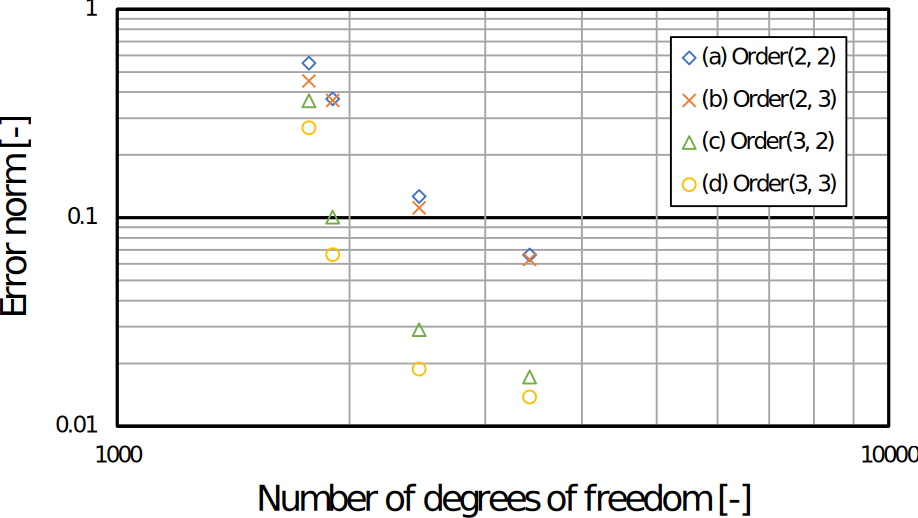
\includegraphics[keepaspectratio, scale=0.5]
  {fig/result_data_etc/s-iga01/r-crop.pdf}
  \caption{Error norm of $\sigma_{rr}$ in each case}
  \label{fig:ERNr}
\end{figure}

\newpage

\begin{figure}[htbp]
  \centering
  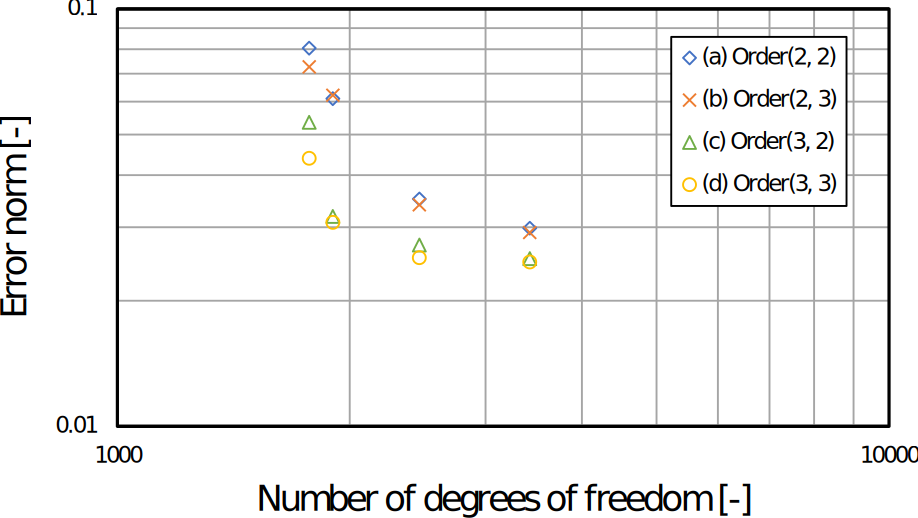
\includegraphics[keepaspectratio, scale=0.5]
  {fig/result_data_etc/s-iga01/theta-crop.pdf}
  \caption{Error norm of $\sigma_{\theta\theta}$ in each case}
  \label{fig:ERNt}
\end{figure}

$y$方向応力$\sigma_{yy}$の応力分布図を図~\ref{fig:contour22}~図~\ref{fig:contour33}に示す.

\begin{figure}[htbp]
  \begin{tabular}{cc}
    \begin{minipage}[t]{0.45\hsize}
      \centering
      \includegraphics[keepaspectratio, scale=0.3]
      {fig/result_data_etc/s-iga01/contour/2_2.png}
      \caption{Stress in $y$ direction on Local patch ((a) Order(2, 2), Control points on Local patch $30\times 30$)}
      \label{fig:contour22}
    \end{minipage} &
    \begin{minipage}[t]{0.45\hsize}
      \centering
      \includegraphics[keepaspectratio, scale=0.3]
      {fig/result_data_etc/s-iga01/contour/2_3.png}
      \caption{Stress in $y$ direction on Local patch ((b) Order(2, 3), Control points on Local patch $30\times 30$)}
      \label{fig:contour23}
    \end{minipage}
  \end{tabular}
\end{figure}

\newpage

\begin{figure}[htbp]
  \begin{tabular}{cc}
    \begin{minipage}[t]{0.45\hsize}
      \centering
      \includegraphics[keepaspectratio, scale=0.3]
      {fig/result_data_etc/s-iga01/contour/3_2.png}
      \caption{Stress in $y$ direction on Local patch ((c) Order(3, 2), Control points on Local patch $30\times 30$)}
      \label{fig:contour32}
    \end{minipage} &
    \begin{minipage}[t]{0.45\hsize}
      \centering
      \includegraphics[keepaspectratio, scale=0.3]
      {fig/result_data_etc/s-iga01/contour/3_3.png}
      \caption{Stress in $y$ direction on Local patch ((d) Order(3, 3), Control points on Local patch $30\times 30$)}
      \label{fig:contour33}
    \end{minipage}
  \end{tabular}
\end{figure}

\newpage

\subsubsection{グローバルパッチの分割数を固定してローカルパッチの分割数を変更した解析}
グローバルパッチのコントロールポイントの分割数を固定してローカルパッチのコントロールポイントの分割数を
変更した重合パッチ法解析を行った.
グローバルパッチとローカルパッチの基底関数が共に2次の場合と共に3次の場合で解析を行い比較した.
グローバルパッチとローカルパッチは
2次の基底関数を用いた場合と3次の基底関数を用いた場合で,
パラメータ空間の各方向に対してコントロールポイント数が等しく,
各方向のコントロールポイントの分割数を変更した重合パッチ法解析モデルを作成した.
グローバルパッチとローカルパッチの各方向のコントロールポイント数,自由度数,総要素数を表~\ref{table:G fixed}に示す.

\begin{table}[hbtp]
  \caption{Details of S-IGA analytical model (Global patch division is fixed)}
  \label{table:G fixed}
  \centering
  \scalebox{0.8}{
    \begin{tabular}{|c|c|c|c|c|c|c|c|c|}
      \hline
      \begin{tabular}{c}
        Order of basis function \\
        (Global patch and Local patch)
      \end{tabular} & \multicolumn{4}{c|}{2} & \multicolumn{4}{c|}{3} \\
      \hline
      \begin{tabular}{c}
        Control points\\
        on Global patch ($\xi \times \eta$)
      \end{tabular} & \multicolumn{4}{c|}{$30\times 30$} & \multicolumn{4}{c|}{$30\times 30$} \\
      \hline
      \begin{tabular}{c}
        Control points\\
        on Local patch ($\xi \times \eta$)
      \end{tabular} & $5\times 5$ & $10\times 10$ & $20\times 20$ & $30\times 30$ & $5\times 5$ & $10\times 10$ & $20\times 20$ & $30\times 30$ \\
      \hline
      Degrees of freedom & 1772 & 1902 & 2462 & 3422 & 1772 & 1902 & 2462 & 3422 \\
      \hline
      Total elements & 793 & 848 & 1108 & 1568 & 733 & 778 & 1018 & 1458 \\
      \hline
    \end{tabular}
  }
\end{table}

例として,2次の基底関数で,ローカルパッチの分割数を変更した重合パッチ法解析モデルを図~\ref{fig:s-iga02 model01}~
図~\ref{fig:s-iga02 model04}に示す.

\begin{figure}[htbp]
  \begin{tabular}{cc}
    \begin{minipage}[t]{0.45\hsize}
      \centering
      \includegraphics[keepaspectratio, scale=0.3]
      {fig/result_data_etc/s-iga02/model/5x5.png}
      \caption{An example of second-order S-IGA analytical model (Global patch $30\times 30$, Local patch $5\times 5$)}
      \label{fig:s-iga02 model01}
    \end{minipage} &
    \begin{minipage}[t]{0.45\hsize}
      \centering
      \includegraphics[keepaspectratio, scale=0.3]
      {fig/result_data_etc/s-iga02/model/10x10.png}
      \caption{An example of second-order S-IGA analytical model (Global patch $30\times 30$, Local patch $10\times 10$)}
      \label{fig:s-iga02 model02}
    \end{minipage}
  \end{tabular}
\end{figure}

\newpage

\begin{figure}[hbtp]
  \begin{tabular}{cc}
    \begin{minipage}[t]{0.45\hsize}
      \centering
      \includegraphics[keepaspectratio, scale=0.3]
      {fig/result_data_etc/s-iga02/model/20x20.png}
      \caption{An example of second-order S-IGA analytical model (Global patch $30\times 30$, Local patch $20\times 20$)}
      \label{fig:s-iga02 model03}
    \end{minipage} &
    \begin{minipage}[t]{0.45\hsize}
      \centering
      \includegraphics[keepaspectratio, scale=0.3]
      {fig/result_data_etc/s-iga02/model/30x30.png}
      \caption{An example of second-order S-IGA analytical model (Global patch $30\times 30$, Local patch $30\times 30$)}
      \label{fig:s-iga02 model04}
    \end{minipage}
  \end{tabular}
\end{figure}

\noindent
以上の解析モデルについて解析を行い,精度検証を行った.
円孔縁の主応力$\sigma_1, \sigma_2$の分布,$x$軸上の$y$方向応力$\sigma_{yy}$,応力分布図を比較し,
ローカルパッチの分割数による影響を比較した.

円孔縁の主応力$\sigma_1, \sigma_2$の分布を
図~\ref{fig:s-iga02 s 2 5x5}~図~\ref{fig:s-iga02 s 3 30x30}に示す.

\begin{figure}[hbtp]
  \begin{tabular}{cc}
    \begin{minipage}[t]{0.45\hsize}
      \centering
      \includegraphics[keepaspectratio, scale=0.4]
      {fig/result_data_etc/s-iga02/order2/s_5x5-crop.pdf}
      \caption{Principal stress along the periphery of the circular hole (second-order, Global patch $30\times 30$, Local patch $5\times 5$)}
      \label{fig:s-iga02 s 2 5x5}
    \end{minipage} &
    \begin{minipage}[t]{0.45\hsize}
      \centering
      \includegraphics[keepaspectratio, scale=0.4]
      {fig/result_data_etc/s-iga02/order3/s_5x5-crop.pdf}
      \caption{Principal stress along the periphery of the circular hole (third-order, Global patch $30\times 30$, Local patch $5\times 5$)}
      \label{fig:s-iga02 s 3 5x5}
    \end{minipage}
  \end{tabular}
\end{figure}

\newpage

\begin{figure}[hbtp]
  \begin{tabular}{cc}
    \begin{minipage}[t]{0.45\hsize}
      \centering
      \includegraphics[keepaspectratio, scale=0.4]
      {fig/result_data_etc/s-iga02/order2/s_10x10-crop.pdf}
      \caption{Principal stress along the periphery of the circular hole (second-order, Global patch $30\times 30$, Local patch $10\times 10$)}
      \label{fig:s-iga02 s 2 10x10}
    \end{minipage} &
    \begin{minipage}[t]{0.45\hsize}
      \centering
      \includegraphics[keepaspectratio, scale=0.4]
      {fig/result_data_etc/s-iga02/order3/s_10x10-crop.pdf}
      \caption{Principal stress along the periphery of the circular hole (third-order, Global patch $30\times 30$, Local patch $10\times 10$)}
      \label{fig:s-iga02 s 3 10x10}
    \end{minipage}
  \end{tabular}
\end{figure}

\begin{figure}[hbtp]
  \begin{tabular}{cc}
    \begin{minipage}[t]{0.45\hsize}
      \centering
      \includegraphics[keepaspectratio, scale=0.4]
      {fig/result_data_etc/s-iga02/order2/s_20x20-crop.pdf}
      \caption{Principal stress along the periphery of the circular hole (second-order, Global patch $30\times 30$, Local patch $20\times 20$)}
      \label{fig:s-iga02 s 2 20x20}
    \end{minipage} &
    \begin{minipage}[t]{0.45\hsize}
      \centering
      \includegraphics[keepaspectratio, scale=0.4]
      {fig/result_data_etc/s-iga02/order3/s_20x20-crop.pdf}
      \caption{Principal stress along the periphery of the circular hole (third-order, Global patch $30\times 30$, Local patch $20\times 20$)}
      \label{fig:s-iga02 s 3 20x20}
    \end{minipage}
  \end{tabular}
\end{figure}

\begin{figure}[hbtp]
  \begin{tabular}{cc}
    \begin{minipage}[t]{0.45\hsize}
      \centering
      \includegraphics[keepaspectratio, scale=0.4]
      {fig/result_data_etc/s-iga02/order2/s_30x30-crop.pdf}
      \caption{Principal stress along the periphery of the circular hole (second-order, Global patch $30\times 30$, Local patch $30\times 30$)}
      \label{fig:s-iga02 s 2 30x30}
    \end{minipage} &
    \begin{minipage}[t]{0.45\hsize}
      \centering
      \includegraphics[keepaspectratio, scale=0.4]
      {fig/result_data_etc/s-iga02/order3/s_30x30-crop.pdf}
      \caption{Principal stress along the periphery of the circular hole (third-order, Global patch $30\times 30$, Local patch $30\times 30$)}
      \label{fig:s-iga02 s 3 30x30}
    \end{minipage}
  \end{tabular}
\end{figure}

\newpage

$x$軸上の$y$方向応力$\sigma_{yy}$を
図~\ref{fig:s-iga02 y 2 5x5}~図~\ref{fig:s-iga02 y 3 30x30}に示す.

\begin{figure}[hbtp]
  \begin{tabular}{cc}
    \begin{minipage}[t]{0.45\hsize}
      \centering
      \includegraphics[keepaspectratio, scale=0.4]
      {fig/result_data_etc/s-iga02/order2/y_5x5-crop.pdf}
      \caption{Stress in $y$ direction along the line $y = 0$ (second-order, Global patch $30\times 30$, Local patch $5\times 5$)}
      \label{fig:s-iga02 y 2 5x5}
    \end{minipage} &
    \begin{minipage}[t]{0.45\hsize}
      \centering
      \includegraphics[keepaspectratio, scale=0.4]
      {fig/result_data_etc/s-iga02/order3/y_5x5-crop.pdf}
      \caption{Stress in $y$ direction along the line $y = 0$ (third-order, Global patch $30\times 30$, Local patch $5\times 5$)}
      \label{fig:s-iga02 y 3 5x5}
    \end{minipage}
  \end{tabular}
\end{figure}

\begin{figure}[hbtp]
  \begin{tabular}{cc}
    \begin{minipage}[t]{0.45\hsize}
      \centering
      \includegraphics[keepaspectratio, scale=0.4]
      {fig/result_data_etc/s-iga02/order2/y_10x10-crop.pdf}
      \caption{Stress in $y$ direction along the line $y = 0$ (second-order, Global patch $30\times 30$, Local patch $10\times 10$)}
      \label{fig:s-iga02 y 2 10x10}
    \end{minipage} &
    \begin{minipage}[t]{0.45\hsize}
      \centering
      \includegraphics[keepaspectratio, scale=0.4]
      {fig/result_data_etc/s-iga02/order3/y_10x10-crop.pdf}
      \caption{Stress in $y$ direction along the line $y = 0$ (third-order, Global patch $30\times 30$, Local patch $10\times 10$)}
      \label{fig:s-iga02 y 3 10x10}
    \end{minipage}
  \end{tabular}
\end{figure}

\begin{figure}[hbtp]
  \begin{tabular}{cc}
    \begin{minipage}[t]{0.45\hsize}
      \centering
      \includegraphics[keepaspectratio, scale=0.4]
      {fig/result_data_etc/s-iga02/order2/y_20x20-crop.pdf}
      \caption{Stress in $y$ direction along the line $y = 0$ (second-order, Global patch $30\times 30$, Local patch $20\times 20$)}
      \label{fig:s-iga02 y 2 20x20}
    \end{minipage} &
    \begin{minipage}[t]{0.45\hsize}
      \centering
      \includegraphics[keepaspectratio, scale=0.4]
      {fig/result_data_etc/s-iga02/order3/y_20x20-crop.pdf}
      \caption{Stress in $y$ direction along the line $y = 0$ (third-order, Global patch $30\times 30$, Local patch $20\times 20$)}
      \label{fig:s-iga02 y 3 20x20}
    \end{minipage}
  \end{tabular}
\end{figure}

\newpage

\begin{figure}[hbtp]
  \begin{tabular}{cc}
    \begin{minipage}[t]{0.45\hsize}
      \centering
      \includegraphics[keepaspectratio, scale=0.4]
      {fig/result_data_etc/s-iga02/order2/y_30x30-crop.pdf}
      \caption{Stress in $y$ direction along the line $y = 0$ (second-order, Global patch $30\times 30$, Local patch $30\times 30$)}
      \label{fig:s-iga02 y 2 30x30}
    \end{minipage} &
    \begin{minipage}[t]{0.45\hsize}
      \centering
      \includegraphics[keepaspectratio, scale=0.4]
      {fig/result_data_etc/s-iga02/order3/y_30x30-crop.pdf}
      \caption{Stress in $y$ direction along the line $y = 0$ (third-order, Global patch $30\times 30$, Local patch $30\times 30$)}
      \label{fig:s-iga02 y 3 30x30}
    \end{minipage}
  \end{tabular}
\end{figure}

$y$方向応力$\sigma_{yy}$の分布図を図~\ref{fig:s-iga02 y 2},図~\ref{fig:s-iga02 y 3}に示す.

\begin{figure}[hbtp]
  \begin{tabular}{cc}
    \begin{minipage}[t]{0.45\hsize}
      \centering
      \includegraphics[keepaspectratio, scale=0.3]
      {fig/result_data_etc/s-iga02/contour/2.png}
      \caption{Stress in $y$ direction on Local patch (second-order, Global patch $30\times 30$, Local patch $20\times 20$)}
      \label{fig:s-iga02 y 2}
    \end{minipage} &
    \begin{minipage}[t]{0.45\hsize}
      \centering
      \includegraphics[keepaspectratio, scale=0.3]
      {fig/result_data_etc/s-iga02/contour/3.png}
      \caption{Stress in $y$ direction on Local patch (third-order, Global patch $30\times 30$, Local patch $20\times 20$)}
      \label{fig:s-iga02 y 3}
    \end{minipage}
  \end{tabular}
\end{figure}

\newpage

\subsubsection{ローカルパッチの分割数を固定してグローバルパッチの分割数を変更した解析}
ローカルパッチのコントロールポイントの分割数を固定してグローバルパッチのコントロールポイントの分割数を
変更した重合パッチ法解析を行った.
グローバルパッチとローカルパッチの基底関数が共に2次の場合と共に3次の場合で解析を行い比較した.
グローバルパッチとローカルパッチは
2次の基底関数を用いた場合と3次の基底関数を用いた場合で,
パラメータ空間の各方向に対してコントロールポイント数が等しく,
各方向のコントロールポイントの分割数を変更した重合パッチ法解析モデルを作成した.
グローバルパッチとローカルパッチの各方向のコントロールポイント数,自由度数,総要素数を表~\ref{table:L fixed}に示す.

\begin{table}[hbtp]
  \caption{Details of S-IGA analytical model (Local patch division is fixed)}
  \label{table:L fixed}
  \centering
  \scalebox{0.8}{
    \begin{tabular}{|c|c|c|c|c|c|c|c|c|}
      \hline
      \begin{tabular}{c}
        Order of basis function \\
        (Global patch and Local patch)
      \end{tabular} & \multicolumn{4}{c|}{2} & \multicolumn{4}{c|}{3} \\
      \hline
      \begin{tabular}{c}
        Control points\\
        on Local patch ($\xi \times \eta$)
      \end{tabular} & \multicolumn{4}{c|}{$30\times 30$} & \multicolumn{4}{c|}{$30\times 30$} \\
      \hline
      \begin{tabular}{c}
        Control points\\
        on Global patch ($\xi \times \eta$)
      \end{tabular} & $5\times 5$ & $10\times 10$ & $20\times 20$ & $30\times 30$ & $5\times 5$ & $10\times 10$ & $20\times 20$ & $30\times 30$ \\
      \hline
      Degrees of freedom & 1722 & 1862 & 2442 & 3422 & 1722 & 1862 & 2442 & 3422 \\
      \hline
      Total elements & 793 & 848 & 1108 & 1568 & 733 & 778 & 1018 & 1458 \\
      \hline
    \end{tabular}
  }
\end{table}

例として,2次の基底関数で,グローバルパッチの分割数を変更した重合パッチ法解析モデルを図~\ref{fig:s-iga03 model01}~
図~\ref{fig:s-iga03 model04}に示す.

\begin{figure}[htbp]
  \begin{tabular}{cc}
    \begin{minipage}[t]{0.45\hsize}
      \centering
      \includegraphics[keepaspectratio, scale=0.3]
      {fig/result_data_etc/s-iga03/model/5x5.png}
      \caption{An example of second-order S-IGA analytical model (Global patch $5\times 5$, Local patch $30\times 30$)}
      \label{fig:s-iga03 model01}
    \end{minipage} &
    \begin{minipage}[t]{0.45\hsize}
      \centering
      \includegraphics[keepaspectratio, scale=0.3]
      {fig/result_data_etc/s-iga03/model/10x10.png}
      \caption{An example of second-order S-IGA analytical model (Global patch $10\times 10$, Local patch $30\times 30$)}
      \label{fig:s-iga03 model02}
    \end{minipage}
  \end{tabular}
\end{figure}

\newpage

\begin{figure}[htbp]
  \begin{tabular}{cc}
    \begin{minipage}[t]{0.45\hsize}
      \centering
      \includegraphics[keepaspectratio, scale=0.3]
      {fig/result_data_etc/s-iga03/model/20x20.png}
      \caption{An example of second-order S-IGA analytical model (Global patch $20\times 20$, Local patch $30\times 30$)}
      \label{fig:s-iga03 model03}
    \end{minipage} &
    \begin{minipage}[t]{0.45\hsize}
      \centering
      \includegraphics[keepaspectratio, scale=0.3]
      {fig/result_data_etc/s-iga03/model/30x30.png}
      \caption{An example of second-order S-IGA analytical model (Global patch $30\times 30$, Local patch $30\times 30$)}
      \label{fig:s-iga03 model04}
    \end{minipage}
  \end{tabular}
\end{figure}

\noindent
以上の解析モデルについて解析を行い,精度検証を行った.
円孔縁の主応力$\sigma_1, \sigma_2$の分布,$x$軸上の$y$方向応力$\sigma_{yy}$,応力分布図を比較し,
グローバルパッチの分割数による影響を比較した.

円孔縁の主応力$\sigma_1, \sigma_2$の分布を
図~\ref{fig:s-iga03 s 2 5x5}~図~\ref{fig:s-iga03 s 3 30x30}に示す.

\begin{figure}[hbtp]
  \begin{tabular}{cc}
    \begin{minipage}[t]{0.45\hsize}
      \centering
      \includegraphics[keepaspectratio, scale=0.4]
      {fig/result_data_etc/s-iga03/order2/s_5x5-crop.pdf}
      \caption{Principal stress along the periphery of the circular hole (second-order, Global patch $5\times 5$, Local patch $30\times 30$)}
      \label{fig:s-iga03 s 2 5x5}
    \end{minipage} &
    \begin{minipage}[t]{0.45\hsize}
      \centering
      \includegraphics[keepaspectratio, scale=0.4]
      {fig/result_data_etc/s-iga03/order3/s_5x5-crop.pdf}
      \caption{Principal stress along the periphery of the circular hole (third-order, Global patch $5\times 5$, Local patch $30\times 30$)}
      \label{fig:s-iga03 s 3 5x5}
    \end{minipage}
  \end{tabular}
\end{figure}

\newpage

\begin{figure}[hbtp]
  \begin{tabular}{cc}
    \begin{minipage}[t]{0.45\hsize}
      \centering
      \includegraphics[keepaspectratio, scale=0.4]
      {fig/result_data_etc/s-iga03/order2/s_10x10-crop.pdf}
      \caption{Principal stress along the periphery of the circular hole (second-order, Global patch $10\times 10$, Local patch $30\times 30$)}
      \label{fig:s-iga03 s 2 10x10}
    \end{minipage} &
    \begin{minipage}[t]{0.45\hsize}
      \centering
      \includegraphics[keepaspectratio, scale=0.4]
      {fig/result_data_etc/s-iga03/order3/s_10x10-crop.pdf}
      \caption{Principal stress along the periphery of the circular hole (third-order, Global patch $10\times 10$, Local patch $30\times 30$)}
      \label{fig:s-iga03 s 3 10x10}
    \end{minipage}
  \end{tabular}
\end{figure}

\begin{figure}[hbtp]
  \begin{tabular}{cc}
    \begin{minipage}[t]{0.45\hsize}
      \centering
      \includegraphics[keepaspectratio, scale=0.4]
      {fig/result_data_etc/s-iga03/order2/s_20x20-crop.pdf}
      \caption{Principal stress along the periphery of the circular hole (second-order, Global patch $20\times 20$, Local patch $30\times 30$)}
      \label{fig:s-iga03 s 2 20x20}
    \end{minipage} &
    \begin{minipage}[t]{0.45\hsize}
      \centering
      \includegraphics[keepaspectratio, scale=0.4]
      {fig/result_data_etc/s-iga03/order3/s_20x20-crop.pdf}
      \caption{Principal stress along the periphery of the circular hole (third-order, Global patch $20\times 20$, Local patch $30\times 30$)}
      \label{fig:s-iga03 s 3 20x20}
    \end{minipage}
  \end{tabular}
\end{figure}

\begin{figure}[hbtp]
  \begin{tabular}{cc}
    \begin{minipage}[t]{0.45\hsize}
      \centering
      \includegraphics[keepaspectratio, scale=0.4]
      {fig/result_data_etc/s-iga03/order2/s_30x30-crop.pdf}
      \caption{Principal stress along the periphery of the circular hole (second-order, Global patch $30\times 30$, Local patch $30\times 30$)}
      \label{fig:s-iga03 s 2 30x30}
    \end{minipage} &
    \begin{minipage}[t]{0.45\hsize}
      \centering
      \includegraphics[keepaspectratio, scale=0.4]
      {fig/result_data_etc/s-iga03/order3/s_30x30-crop.pdf}
      \caption{Principal stress along the periphery of the circular hole (third-order, Global patch $30\times 30$, Local patch $30\times 30$)}
      \label{fig:s-iga03 s 3 30x30}
    \end{minipage}
  \end{tabular}
\end{figure}

\newpage

$x$軸上の$y$方向応力$\sigma_{yy}$を
図~\ref{fig:s-iga03 y 2 5x5}~図~\ref{fig:s-iga03 y 3 30x30}に示す.

\begin{figure}[hbtp]
  \begin{tabular}{cc}
    \begin{minipage}[t]{0.45\hsize}
      \centering
      \includegraphics[keepaspectratio, scale=0.4]
      {fig/result_data_etc/s-iga03/order2/y_5x5-crop.pdf}
      \caption{Stress in $y$ direction along the line $y = 0$ (second-order, Global patch $5\times 5$, Local patch $30\times 30$)}
      \label{fig:s-iga03 y 2 5x5}
    \end{minipage} &
    \begin{minipage}[t]{0.45\hsize}
      \centering
      \includegraphics[keepaspectratio, scale=0.4]
      {fig/result_data_etc/s-iga03/order3/y_5x5-crop.pdf}
      \caption{Stress in $y$ direction along the line $y = 0$ (third-order, Global patch $5\times 5$, Local patch $30\times 30$)}
      \label{fig:s-iga03 y 3 5x5}
    \end{minipage}
  \end{tabular}
\end{figure}

\begin{figure}[hbtp]
  \begin{tabular}{cc}
    \begin{minipage}[t]{0.45\hsize}
      \centering
      \includegraphics[keepaspectratio, scale=0.4]
      {fig/result_data_etc/s-iga03/order2/y_10x10-crop.pdf}
      \caption{Stress in $y$ direction along the line $y = 0$ (second-order, Global patch $10\times 10$, Local patch $30\times 30$)}
      \label{fig:s-iga03 y 2 10x10}
    \end{minipage} &
    \begin{minipage}[t]{0.45\hsize}
      \centering
      \includegraphics[keepaspectratio, scale=0.4]
      {fig/result_data_etc/s-iga03/order3/y_10x10-crop.pdf}
      \caption{Stress in $y$ direction along the line $y = 0$ (third-order, Global patch $10\times 10$, Local patch $30\times 30$)}
      \label{fig:s-iga03 y 3 10x10}
    \end{minipage}
  \end{tabular}
\end{figure}

\begin{figure}[hbtp]
  \begin{tabular}{cc}
    \begin{minipage}[t]{0.45\hsize}
      \centering
      \includegraphics[keepaspectratio, scale=0.4]
      {fig/result_data_etc/s-iga03/order2/y_20x20-crop.pdf}
      \caption{Stress in $y$ direction along the line $y = 0$ (second-order, Global patch $20\times 20$, Local patch $30\times 30$)}
      \label{fig:s-iga03 y 2 20x20}
    \end{minipage} &
    \begin{minipage}[t]{0.45\hsize}
      \centering
      \includegraphics[keepaspectratio, scale=0.4]
      {fig/result_data_etc/s-iga03/order3/y_20x20-crop.pdf}
      \caption{Stress in $y$ direction along the line $y = 0$ (third-order, Global patch $20\times 20$, Local patch $30\times 30$)}
      \label{fig:s-iga03 y 3 20x20}
    \end{minipage}
  \end{tabular}
\end{figure}

\newpage

\begin{figure}[hbtp]
  \begin{tabular}{cc}
    \begin{minipage}[t]{0.45\hsize}
      \centering
      \includegraphics[keepaspectratio, scale=0.4]
      {fig/result_data_etc/s-iga03/order2/y_30x30-crop.pdf}
      \caption{Stress in $y$ direction along the line $y = 0$ (second-order, Global patch $30\times 30$, Local patch $30\times 30$)}
      \label{fig:s-iga03 y 2 30x30}
    \end{minipage} &
    \begin{minipage}[t]{0.45\hsize}
      \centering
      \includegraphics[keepaspectratio, scale=0.4]
      {fig/result_data_etc/s-iga03/order3/y_30x30-crop.pdf}
      \caption{Stress in $y$ direction along the line $y = 0$ (third-order, Global patch $30\times 30$, Local patch $30\times 30$)}
      \label{fig:s-iga03 y 3 30x30}
    \end{minipage}
  \end{tabular}
\end{figure}

$y$方向応力$\sigma_{yy}$の分布図を図~\ref{fig:s-iga03 y 2},図~\ref{fig:s-iga03 y 3}に示す.

\begin{figure}[hbtp]
  \begin{tabular}{cc}
    \begin{minipage}[t]{0.45\hsize}
      \centering
      \includegraphics[keepaspectratio, scale=0.3]
      {fig/result_data_etc/s-iga03/contour/2.png}
      \caption{Stress in $y$ direction on Local patch (second-order, Global patch $20\times 20$, Local patch $30\times 30$)}
      \label{fig:s-iga03 y 2}
    \end{minipage} &
    \begin{minipage}[t]{0.45\hsize}
      \centering
      \includegraphics[keepaspectratio, scale=0.3]
      {fig/result_data_etc/s-iga03/contour/3.png}
      \caption{Stress in $y$ direction on Local patch (third-order, Global patch $20\times 20$, Local patch $30\times 30$)}
      \label{fig:s-iga03 y 3}
    \end{minipage}
  \end{tabular}
\end{figure}

\newpage

\subsubsection{グローバルパッチの分割数を固定してローカルパッチのサイズと分割数を変更した解析}
グローバルパッチのコントロールポイントの分割数を固定してローカルパッチの全体のサイズと
コントロールポイントの分割数を変更した重合パッチ法解析を行った.
グローバルパッチとローカルパッチの基底関数が共に2次の場合と共に3次の場合で解析を行い比較した.
表~\ref{table:G fixed}に示すようにグローバルパッチの分割数を固定してローカルパッチの分割数を変更した.
さらに表~\ref{table:L size}に示すようにローカルパッチの全体のサイズを変更した.
図~\ref{fig:r1 r2}に示すようにローカルパッチの内径$2r_1\ $mm,外径$2r_2\ $mmとした.

\begin{table}[hbtp]
  \caption{Local patch size of S-IGA analytical model}
  \label{table:L size}
  \centering
  \scalebox{1.0}{
    \begin{tabular}{|c|c|c|c|c|c|c|}
      \hline
      $r_1$ [mm] & \multicolumn{6}{c|}{1.00} \\
      \hline
      $r_2$ [mm] & 1.25 & 1.50 & 1.75 & 2.00 & 2.25 & 2.50 \\
      \hline
    \end{tabular}
  }
\end{table}

\begin{figure}[htbp]
  \centering
  \includegraphics[keepaspectratio, scale = 0.85]
  {fig/r2.ai}
  \caption{Definition of $r_1$ and $r_2$ on Local patch}
  \label{fig:r1 r2}
\end{figure}

\newpage

例として,2次の基底関数で,ローカルパッチの全体のサイズを変更した重合パッチ法解析モデルを
図~\ref{fig:s-iga04 model 1.25}~図~\ref{fig:s-iga04 model 2.50}に示す.

\begin{figure}[hbtp]
  \begin{tabular}{cc}
    \begin{minipage}[t]{0.45\hsize}
      \centering
      \includegraphics[keepaspectratio, scale=0.35]
      {fig/result_data_etc/s-iga04/model/1.25.png}
      \caption{An example of S-IGA analytical model (second-order, Global patch $30\times 30$, Local patch $10\times 10$, $r_2 = 1.25$[mm])}
      \label{fig:s-iga04 model 1.25}
    \end{minipage} &
    \begin{minipage}[t]{0.45\hsize}
      \centering
      \includegraphics[keepaspectratio, scale=0.35]
      {fig/result_data_etc/s-iga04/model/1.50.png}
      \caption{An example of S-IGA analytical model (second-order, Global patch $30\times 30$, Local patch $10\times 10$, $r_2 = 1.50$[mm])}
      \label{fig:s-iga04 model 1.50}
    \end{minipage}
  \end{tabular}
\end{figure}

\begin{figure}[hbtp]
  \begin{tabular}{cc}
    \begin{minipage}[t]{0.45\hsize}
      \centering
      \includegraphics[keepaspectratio, scale=0.35]
      {fig/result_data_etc/s-iga04/model/1.75.png}
      \caption{An example of S-IGA analytical model (second-order, Global patch $30\times 30$, Local patch $10\times 10$, $r_2 = 1.75$[mm])}
      \label{fig:s-iga04 model 1.75}
    \end{minipage} &
    \begin{minipage}[t]{0.45\hsize}
      \centering
      \includegraphics[keepaspectratio, scale=0.35]
      {fig/result_data_etc/s-iga04/model/2.00.png}
      \caption{An example of S-IGA analytical model (second-order, Global patch $30\times 30$, Local patch $10\times 10$, $r_2 = 2.00$[mm])}
      \label{fig:s-iga04 model 2.00}
    \end{minipage}
  \end{tabular}
\end{figure}

\newpage

\begin{figure}[hbtp]
  \begin{tabular}{cc}
    \begin{minipage}[t]{0.45\hsize}
      \centering
      \includegraphics[keepaspectratio, scale=0.35]
      {fig/result_data_etc/s-iga04/model/2.25.png}
      \caption{An example of S-IGA analytical model (second-order, Global patch $30\times 30$, Local patch $10\times 10$, $r_2 = 2.25$[mm])}
      \label{fig:s-iga04 model 2.25}
    \end{minipage} &
    \begin{minipage}[t]{0.45\hsize}
      \centering
      \includegraphics[keepaspectratio, scale=0.35]
      {fig/result_data_etc/s-iga04/model/2.50.png}
      \caption{An example of S-IGA analytical model (second-order, Global patch $30\times 30$, Local patch $10\times 10$, $r_2 = 2.50$[mm])}
      \label{fig:s-iga04 model 2.50}
    \end{minipage}
  \end{tabular}
\end{figure}

\newpage

\noindent
以上の解析モデルについて解析を行った.

各ローカルパッチサイズでの半径方向応力$\sigma_{rr}$の誤差ノルムを
図~\ref{fig:s-iga04 1.25}~図~\ref{fig:s-iga04 2.50}に示す.

\begin{figure}[hbtp]
  \begin{tabular}{cc}
    \begin{minipage}[t]{0.45\hsize}
      \centering
      \includegraphics[keepaspectratio, scale=0.4]
      {fig/result_data_etc/s-iga04/1.25-crop.pdf}
      \caption{Error norm of $\sigma_{rr}$ ($r_2 = 1.25$[mm])}
      \label{fig:s-iga04 1.25}
    \end{minipage} &
    \begin{minipage}[t]{0.45\hsize}
      \centering
      \includegraphics[keepaspectratio, scale=0.4]
      {fig/result_data_etc/s-iga04/1.50-crop.pdf}
      \caption{Error norm of $\sigma_{rr}$ ($r_2 = 1.50$[mm])}
      \label{fig:s-iga04 1.50}
    \end{minipage}
  \end{tabular}
\end{figure}

\begin{figure}[hbtp]
  \begin{tabular}{cc}
    \begin{minipage}[t]{0.45\hsize}
      \centering
      \includegraphics[keepaspectratio, scale=0.4]
      {fig/result_data_etc/s-iga04/1.75-crop.pdf}
      \caption{Error norm of $\sigma_{rr}$ ($r_2 = 1.75$[mm])}
      \label{fig:s-iga04 1.75}
    \end{minipage} &
    \begin{minipage}[t]{0.45\hsize}
      \centering
      \includegraphics[keepaspectratio, scale=0.4]
      {fig/result_data_etc/s-iga04/2.00-crop.pdf}
      \caption{Error norm of $\sigma_{rr}$ ($r_2 = 2.00$[mm])}
      \label{fig:s-iga04 2.00}
    \end{minipage}
  \end{tabular}
\end{figure}

\begin{figure}[hbtp]
  \begin{tabular}{cc}
    \begin{minipage}[t]{0.45\hsize}
      \centering
      \includegraphics[keepaspectratio, scale=0.4]
      {fig/result_data_etc/s-iga04/2.25-crop.pdf}
      \caption{Error norm of $\sigma_{rr}$ ($r_2 = 2.25$[mm])}
      \label{fig:s-iga04 2.25}
    \end{minipage} &
    \begin{minipage}[t]{0.45\hsize}
      \centering
      \includegraphics[keepaspectratio, scale=0.4]
      {fig/result_data_etc/s-iga04/2.50-crop.pdf}
      \caption{Error norm of $\sigma_{rr}$ ($r_2 = 2.50$[mm])}
      \label{fig:s-iga04 2.50}
    \end{minipage}
  \end{tabular}
\end{figure}
